%   ファイルおよびフォルダ名(ディレクトリ名)の表記には\verbコマンドを用いる.
%   引数を持たないコマンドは基本的に波括弧で囲う.(e.g. {\hoge})
%   一行あたりの最大文字数は135文字を目安に折り返す.

\addtocounter{page}{-1}

%%%%%%%%%%%%%%%%%%%%%% §1 %%%%%%%%%%%%%%%%%%%%%%
\chapter{事前準備}

%%%%%%%%%%%%%%%%%%%%% §1.1 %%%%%%%%%%%%%%%%%%%%%
\section{{\TeX}のインストール}

{\ketcindy}は{\TeX}をベースとした教材作成支援システムとして開発された.
そこで,{\ketcindy}をインストールする前に,{\TeX}のインストール手順を説明する.
{\TeX}とは,コンピュータ上で出版物を作成できる組版システムのことである.
{\TeX}のフルスペック版は{\TeX}Liveとして纏められたおり,毎年アップデートされ,最新版は{\TeX}Live2023である.

ところで,{\ketcindy}ではフルスペックの{\TeX}を必要としていないため,最低限必要な部分だけ組み込んだ簡易版としてKeT{\TeX}が開発された.
KeT{\TeX}は1.6GB程度とサイズが小さく,日本語で文書を作成する程度なら全く問題ない.
フルスペック版に拘らなければ,ディスク容量を軽減できるため,KeT{\TeX}がお勧めである.

%%%%%%%%%%%%%%%%%%%% §1.1.1 %%%%%%%%%%%%%%%%%%%%
\subsection{{\TeX}Liveの場合}

\subsubsection{Windowsを使用している場合}
\begin{layer}{180}{0}
    \putnotesw{160}{0}{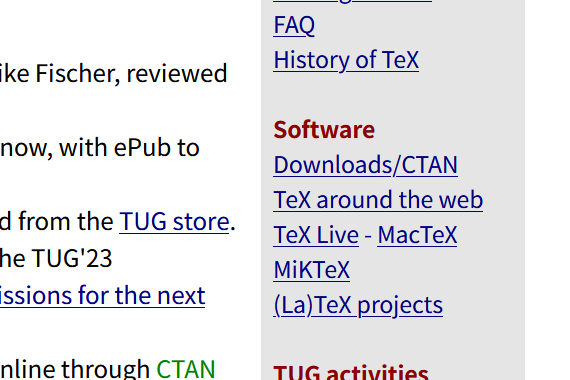
\includegraphics[height=40mm]{./out/fig/texlive-win-1}}
\end{layer}
\begin{enumerate}
    \item \url{https://www.tug.org}にアクセスする
    \item 右ペインにあるSoftwareからTeXLiveを選択する
    \item install on Windowsを選択する
    \item \verb|install-tl-windows.exe|を選択する
    \item exeファイルを管理者として実行\footnote{右クリックメニューから[管理者として実行]を選択}する
    \item インストーラに従いインストールを完了させる
\end{enumerate}
インストール先にCドライブ直下を指定すると{\ketcindy}のインストール時に楽である.

\subsubsection{Macintoshを使用している場合}
Macintoshにおいては,{\TeX}LiveをベースとしてMac{\TeX}という{\TeX}ディストリビューションが開発されている.
ここでは,{\TeX}Liveの代わりにMac{\TeX}のインストール手順を説明する.

\begin{layer}{180}{0}
    \putnotesw{160}{35}{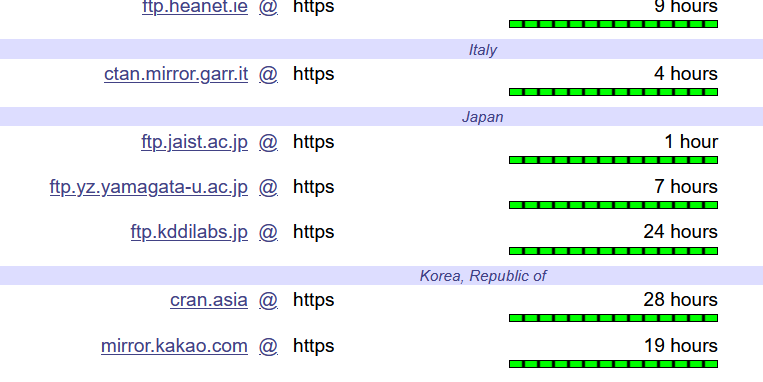
\includegraphics[width=60mm]{./out/fig/texlive-mac-1}}
\end{layer}
\begin{enumerate}
    \item \url{https://tug.org}にアクセスする
    \item 右ペインにあるSoftwareからMacTeXを選択する
    \item MacTeX Download Pageを選択する
    \item 下にスクロールし,Installation Errorsからmirror pageを選択する
    \item www.ctan.org/mirrors/mirmonを選択する
    \item regionsからjpを選択し,最新のミラーを選択する\\
          (画像では,\verb|ftp.jaist.ac.jp|が最新)
    \item 上にスクロールし,MacTeXを選択する
    \item \verb|MacTeX.pkg|を選択する
    \item ダウンロードしたpkgファイルを実行する
    \item インストーラに従いインストールを完了させる
\end{enumerate}

\subsubsection{Linuxを使用している場合}
\begin{enumerate}
    \item \url{https://www.tug.org}にアクセスする
    \item 右ペインにあるSoftwareからTeXLiveを選択する
    \item install on Unix/GNU/Linuxを選択する
    \item tl;dr: Unix(ish)の手順に従いインストールを完了させる
\end{enumerate}

%%%%%%%%%%%%%%%%%%%% §1.1.2 %%%%%%%%%%%%%%%%%%%%
\subsection{KeT{\TeX}の場合}

\subsubsection{Windowsを使用している場合}
\begin{layer}{180}{0}
    \putnotesw{160}{5}{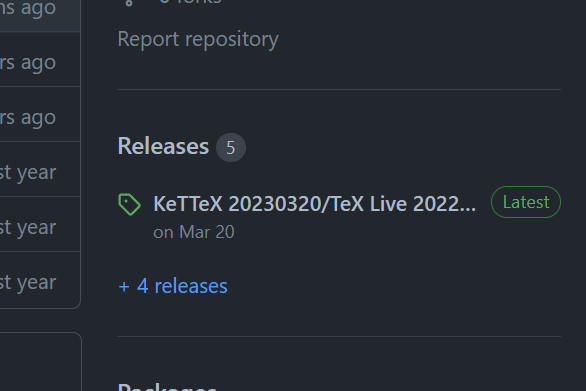
\includegraphics[height=40mm]{./out/fig/kettex-1}}
\end{layer}
\begin{enumerate}
    \item \url{https://github.com/ketpic/kettex}にアクセスする
    \item 右ペインからReleasesを選択する
    \item \verb|KeTTeX-windows-20230320.zip|を選択する
    \item ダウンロードしたzipファイルをCドライブ直下に移動する
    \item zipファイルを解凍しする
    \item 中にある\verb|kettexinst.cmd|を管理者として実行する
    \item インストーラに従いインストールを完了させる
\end{enumerate}

\subsubsection{Macintoshを使用している場合}
\begin{enumerate}
    \item \url{https://github.com/ketpic/kettex}にアクセスする
    \item 右ペインからReleasesを選択する
    \item \verb|KeTTeX-macos-20230320.dmg|を選択する
    \item ダウンロードしたdmgファイル内にある\verb|KeTTeX|を アプリケーション に入れる
\end{enumerate}

\newpage

\subsubsection{Linuxを使用している場合}
\begin{enumerate}
    \item \url{https://github.com/ketpic/kettex}にアクセスする
    \item 右ペインからReleasesを選択する
    \item \verb|KeTTeX-linux-20230320.tar.zst|を選択する
    \item ダウンロードフォルダに移動する
    \item ターミナルから次のコマンドを実行し,ダウンロードしたzstファイルを解凍する
    \begin{lstlisting}
  $ unzstd KeTTeX-linux-20230320.tar.zst
  $ sudo tar xvf KeTTeX-linux-20230320.tar -C /opt
    \end{lstlisting}
\end{enumerate}

%%%%%%%%%%%%%%%%%%%%% §1.2 %%%%%%%%%%%%%%%%%%%%%
\section{周辺ソフトウェアのインストール}

{\ketcindy}は,動的幾何学ソフトCinderellaを用いて図形を描き,{\TeX}の図版ファイルを作るためのシステムである.
gccやMaximaと連携することで,より複雑な処理をすることも可能である.

ここでは,{\ketcindy}と連携できるソフトウェアのインストール手順
\footnote{emathは{\ketcindy}と一緒にインストールするため,ダウンロード手順のみ示す}を説明する.

連携ソフトウェア\footnote{太字のものは必須}およびURLの一覧を下に示す.

\begin{table}[h]
    \centering
    \caption{連携ソフトウェア一覧}
    \label{tab:download}
    \begin{tabular}{c||l}
        \textbf{R}           & \url{https://cran.r-project.org/}\\
        \textbf{Cinderella}  & \url{https://cinderella.de/tiki-index.php}\\
        Maxima      & \url{https://maxima.sourceforge.io/}\\
        MinGW-w64   & \url{https://www.mingw-w64.org/}\\
        emath       & \url{http://emath.s40.xrea.com/}\\
        SumatraPDF  & \url{https://www.sumatrapdfreader.org/free-pdf-reader}
    \end{tabular}
\end{table}

%%%%%%%%%%%%%%%%%%%% §1.2.1 %%%%%%%%%%%%%%%%%%%%
\subsection{Windowsの場合}

ここでは,64bit版Windows 11 Pro (22H2)における連携ソフトウェアのインストール手順を説明する.
特に説明されていない限り,インストール先フォルダは\verb|C:\Program Files|または\verb|C:\Program Files (x86)|を推奨する.

\subsubsection{Rのインストール}
\begin{enumerate}
    \item 表\ref{tab:download}のURLにアクセスする
    \item Download R for Windows→baseと進む
    \item Download R-4.2.3 for Windowsを選択する
    \item ダウンロードしたexeファイルを実行する
    \item インストーラに従いインストールを完了させる
\end{enumerate}

\newpage

\subsubsection{Cinderellaのインストール}
\begin{enumerate}
    \item 表\ref{tab:download}のURLにアクセスする
    \item 右ペインから ダウンロード を選択する
    \item beta.cinderella.deを選択する
    \item Windows 64 Bit Installerを選択する
    \item ダウンロードしたexeファイルを管理者として実行する
    \item インストーラに従いインストールを完了させる
\end{enumerate}

\subsubsection{Maximaのインストール}
\begin{layer}{180}{0}
    \putnotesw{160}{5}{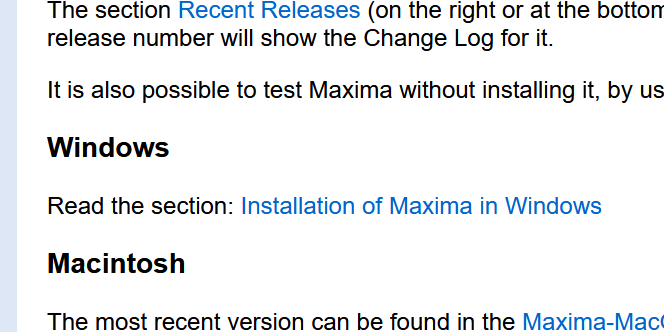
\includegraphics[height=25mm]{./out/fig/maxima-win-1}}
\end{layer}
\begin{enumerate}
    \item 表\ref{tab:download}のURLにアクセスする
    \item 右ペインからDownloadsを選択する
    \item Installation of Maxima in Windows→5.47.0-Windowsと進む
    \item \verb|maxima-5.46.0-win64.exe|を選択する
    \item ダウンロードしたexeファイルを管理者として実行する
    \item インストーラに従いインストールを完了させる
\end{enumerate}

\subsubsection{MinGW-w64のインストール}
\begin{layer}{180}{0}
    \putnotenw{160}{25}{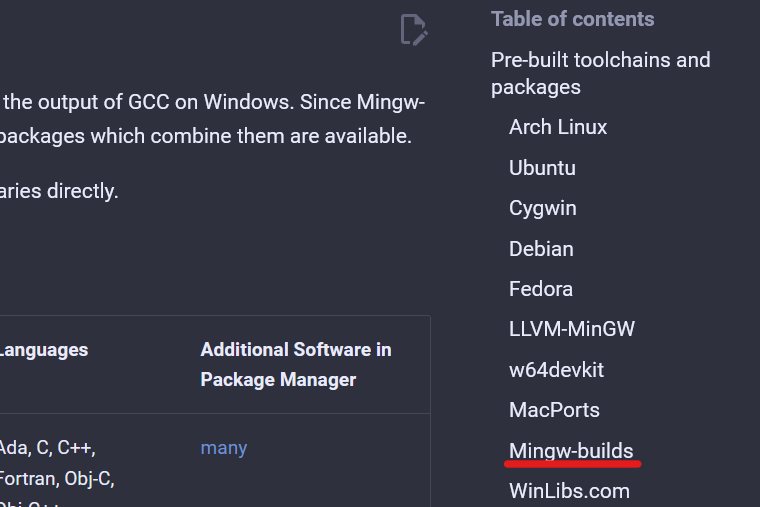
\includegraphics[width=50mm]{./out/fig/c-win-1}}
\end{layer}
\begin{enumerate}
    \item 表\ref{tab:download}のURLにアクセスする
    \item 左ペインからDownloadsを選択する
    \item 右ペインからMingw-buildsを選択する
    \item GitHubを選択する
    \item \verb|x86_64-12.2.0-release-posix-seh-ucrt-rt_v10-rev2.7z|を選択する
    \item ダウンロードした7zファイルを解凍する
    \item 中にある\verb|bin|フォルダの絶対パスをシステム環境変数として登録する
\end{enumerate}

\subsubsection{emathのインストール}
\begin{enumerate}
    \item 表\ref{tab:download}のURLにアクセスする
    \item こちら→入口→丸ごとパック と進む
    \item \verb|emathf051107c.zip|を選択する
\end{enumerate}

\newpage

\subsubsection{PDFビューアのインストール}
ここではSumatraPDFをインストールする.Adobe Acrobat等のPDFビューアも使用可能だが,
PDFファイルを開いている間にファイルがロックされない\footnote{PDFファイルを開いていても外部でファイルの編集ができる}ため,
特にこだわりがなければSumatraPDFがお薦めである.
\begin{enumerate}
    \item 表\ref{tab:download}のURLにアクセスする
    \item Downloadを選択する
    \item \verb|SumatraPDF-3.4.6-64-install.exe|を選択する
    \item ダウンロードしたexeファイルを実行する
    \item インストール先フォルダを\verb|C:\Program Files\SumatraPDF|に変更する
    \item インストーラに従いインストールを完了させる
\end{enumerate}

%%%%%%%%%%%%%%%%%%%% §1.2.2 %%%%%%%%%%%%%%%%%%%%
\subsection{Macintoshの場合}

ここでは,Apple M2 MacBook Air (Ventura 13.1)における連携ソフトウェアのインストール手順を説明する.

\subsubsection{Rのインストール}
\begin{enumerate}
    \item 表\ref{tab:download}のURLにアクセスする
    \item Download R for macOSを選択する
    \item \verb|R-4.2.3-arm64.pkg|を選択する
    \item ダウンロードしたpkgファイルを実行する
    \item インストーラに従いインストールを完了させる
\end{enumerate}

\subsubsection{Cinderellaのインストール}
\begin{enumerate}
    \item 表\ref{tab:download}のURLにアクセスする
    \item 右ペインから ダウンロード を選択する
    \item disk imageを選択する
    \item ダウンロードしたdmgファイル内にある\verb|Cinderella|を アプリケーション に入れる
\end{enumerate}

\subsubsection{Maximaのインストール}
\begin{enumerate}
    \item 表\ref{tab:download}のURLにアクセスする
    \item 右ペインからDownloadsを選択する
    \item Maxima-MacOS download section→5.43.0-MacOSXと進む
    \item \verb|Maxima-5.43.0-VTK-macOS.dmg|を選択する
    \item ダウンロードしたdmgファイル内にある\verb|Maxima|を アプリケーション に入れる
    \item Finderから アプリケーション 内にあるMaximaを探し,controlキーを押しながらクリックする
    \item 開く を選択し,セキュリティ警告を消す
\end{enumerate}

\newpage

\subsubsection{gccのインストール}
\begin{enumerate}
    \item ターミナルから次のコマンドを実行する
          \begin{lstlisting}
  $ sudo xcode-select --install
          \end{lstlisting}
\end{enumerate}

\subsubsection{emathのインストール}
\begin{enumerate}
    \item 表\ref{tab:download}のURLにアクセスする
    \item こちら→入口→丸ごとパック と進む
    \item \verb|emathf051107c.zip|を選択する
\end{enumerate}

%%%%%%%%%%%%%%%%%%%% §1.2.3 %%%%%%%%%%%%%%%%%%%%
\subsection{Linuxの場合}

ここでは,Ubuntu 22.04.2 LTS x86\_64における連携ソフトウェアのインストール手順を説明する.

\subsubsection{Rのインストール}
\begin{enumerate}
    \item 表\ref{tab:download}のURLにアクセスする
    \item Download R for LinuxからUbuntuを選択する
    \item 指示に従いインストールを完了させる
\end{enumerate}

\subsubsection{Cinderellaのインストール}
\begin{enumerate}
    \item 表\ref{tab:download}のURLにアクセスする
    \item 右ペインから ダウンロード を選択する
    \item beta.cinderella.deを選択する
    \item Unix installerを選択する
    \item ダウンロードフォルダに移動する
    \item ダウンロードしたshファイルに実行権限を与え,実行する
    \item インストーラに従いインストールを完了させる
\end{enumerate}

\subsubsection{Maximaのインストール}
\begin{enumerate}
    \item 表\ref{tab:download}のURLにアクセスする
    \item 右ペインからDownloadsを選択する
    \item Using a Linux Packageからthis linkを選択する
    \item ダイアログからAptURLを選択して,Openをクリックする
    \item インストーラに従いインストールを完了させる
\end{enumerate}

\subsubsection{gccのインストール}
\begin{enumerate}
    \item ターミナルから次のコマンドを実行する
    \begin{lstlisting}
  $ sudo apt install gcc
    \end{lstlisting}
\end{enumerate}

\newpage

\subsubsection{emathのインストール}
\begin{enumerate}
    \item 表\ref{tab:download}のURLにアクセスする
    \item こちら→入口→丸ごとパック と進む
    \item \verb|emathf051107c.zip|を選択する
\end{enumerate}
